% A skeleton file for producing Computer Engineering reports
% https://github.com/DeepHorizons/KGCOEReport_template

\documentclass[CMPE]{KGCOEReport}

% The following should be changed to represent your personal information
\newcommand{\classCode}{CMPE 460}  % 4 char code with number
\newcommand{\name}{Jacob Meyerson}
\newcommand{\LabSectionNum}{2}
\newcommand{\LabInstructor}{Professor Beato}	
\newcommand{\TAs}{Brunon Sztuba \\ Eri Montano \\ Connor Henley}
\newcommand{\LectureSectionNum}{1}
\newcommand{\LectureInstructor}{Professor Beato}
\newcommand{\exerciseNumber}{4}
\newcommand{\exerciseDescription}{UART Over Bluetooth}
\newcommand{\dateDone}{February 19, 2021}
\newcommand{\dateSubmitted}{February 26, 2021}

\usepackage{float}
\usepackage{titlesec}
\usepackage{pdfpages}

\begin{document}
\maketitle

\iffalse % No table of contents or other sections for a worksheet -------------------------------------------------
\tableofcontents	%Make a table of contents for all of the sections
\newpage			%New page after table of contents

%Abstract Section
\section*{Abstract}
\addcontentsline{toc}{section}{Abstract}
		
%Design Methodology Section
\section*{Design Methodology}
\addcontentsline{toc}{section}{Design Methodology}

%Results Section	
\section*{Results \& Analysis}
\addcontentsline{toc}{section}{Results \& Analysis}

%Conclusion Section
\section*{Conclusion}
\addcontentsline{toc}{section}{Conclusion}

\fi % -------------------------------------------------------------------------------------------------------------------------------
\section*{Lab Description}
The purpose of this lab is to implement UART through an HM-10 bluetooth module from the K64 boards. UART was initialized for both UART0 through USB and UART3 through bluetooth, and then the two connections interacted with each other in the form of a simple chatroom, where messages could be sent from one device to another. 

\section*{High Level Description of Code}
The first part of the lab required using UART over Bluetooth to control the on board LED. When a 0 was sent, the LED was turned off, when a '1' was sent, the LED turned red, when a '2' was sent, the LED turned blue, and when a '3' was sent, the LED turned green. Any other character or character sequence prompted a message of "Invalid input" to be sent via the Bluetooth UART to the user. This was accomplished using an infinite loop and a switch statement, choosing cases based on the character received. The default case handled the "Invalid Input" case, since any character not '0', '1', '2', or '3' would be considered invalid. The state of the LED was sent via bluetooth to the user on the mobile device. The Bluetooth UART was initialized over UART3 and an HM10 Bluetooth module. UART0 was also initialized to print the status of the LED on the serial console. \\

The chatroom code had 2 separate UARTs initialized, one for USB UART (UART0) and one for Bluetooth UART (UART3). The main loop handled the I/O for both UARTs, seemingly simultaneously but not actually. An infinite loop was run, and in that loop there were 2 if statements. Each if statement was responsible for checking to see if data was coming from a UART device, and was done by polling each UART's RDRF status bit. When the bit was high, a character was available to be read from the UARTx\_D register. Based on this character, there were 3 options. If the character was a carriage return or line feed (Enter key), then a message was displayed from that user in the chat on both screens, for both users to view. This also required emptying the buffer from the sender. If the character was a backspace, then the previous character (if a previous character exists) in the user's buffer was removed, and the character was also removed from the terminal window. For all other cases, the character was added to the user's input buffer, provided the buffer is not full. The code very quickly cycled between checking each UART's RDRF status bit and looked for incoming characters. 

\section*{In Lab Question}
The control loop was implemented as an infinite loop with 2 if statements. Each if statement corresponded to a UART, so one corresponded to UART0 and the other corresponded to UART3. These if statements worked as the getchar conditions, and polled the RDRF flags in both UARTs to see if they were high and have received a character. Then, if a character was received, it got copied from the UARTx\_D register, and handled accordingly (whether it is an Enter, Backspace, or other character). The reason that the control loop could handle both inputs "simultaneously" is because it alternated between polling each UART's RDRF status bit. The input from the USB UART (UART0) was checked, and then the input from the Bluetooth UART (UART3) was checked. Then the loop repeated. This way, it appeared as if both inputs were being handled "simultaneously", but were really handled sequentially, just very quickly. 


\newpage
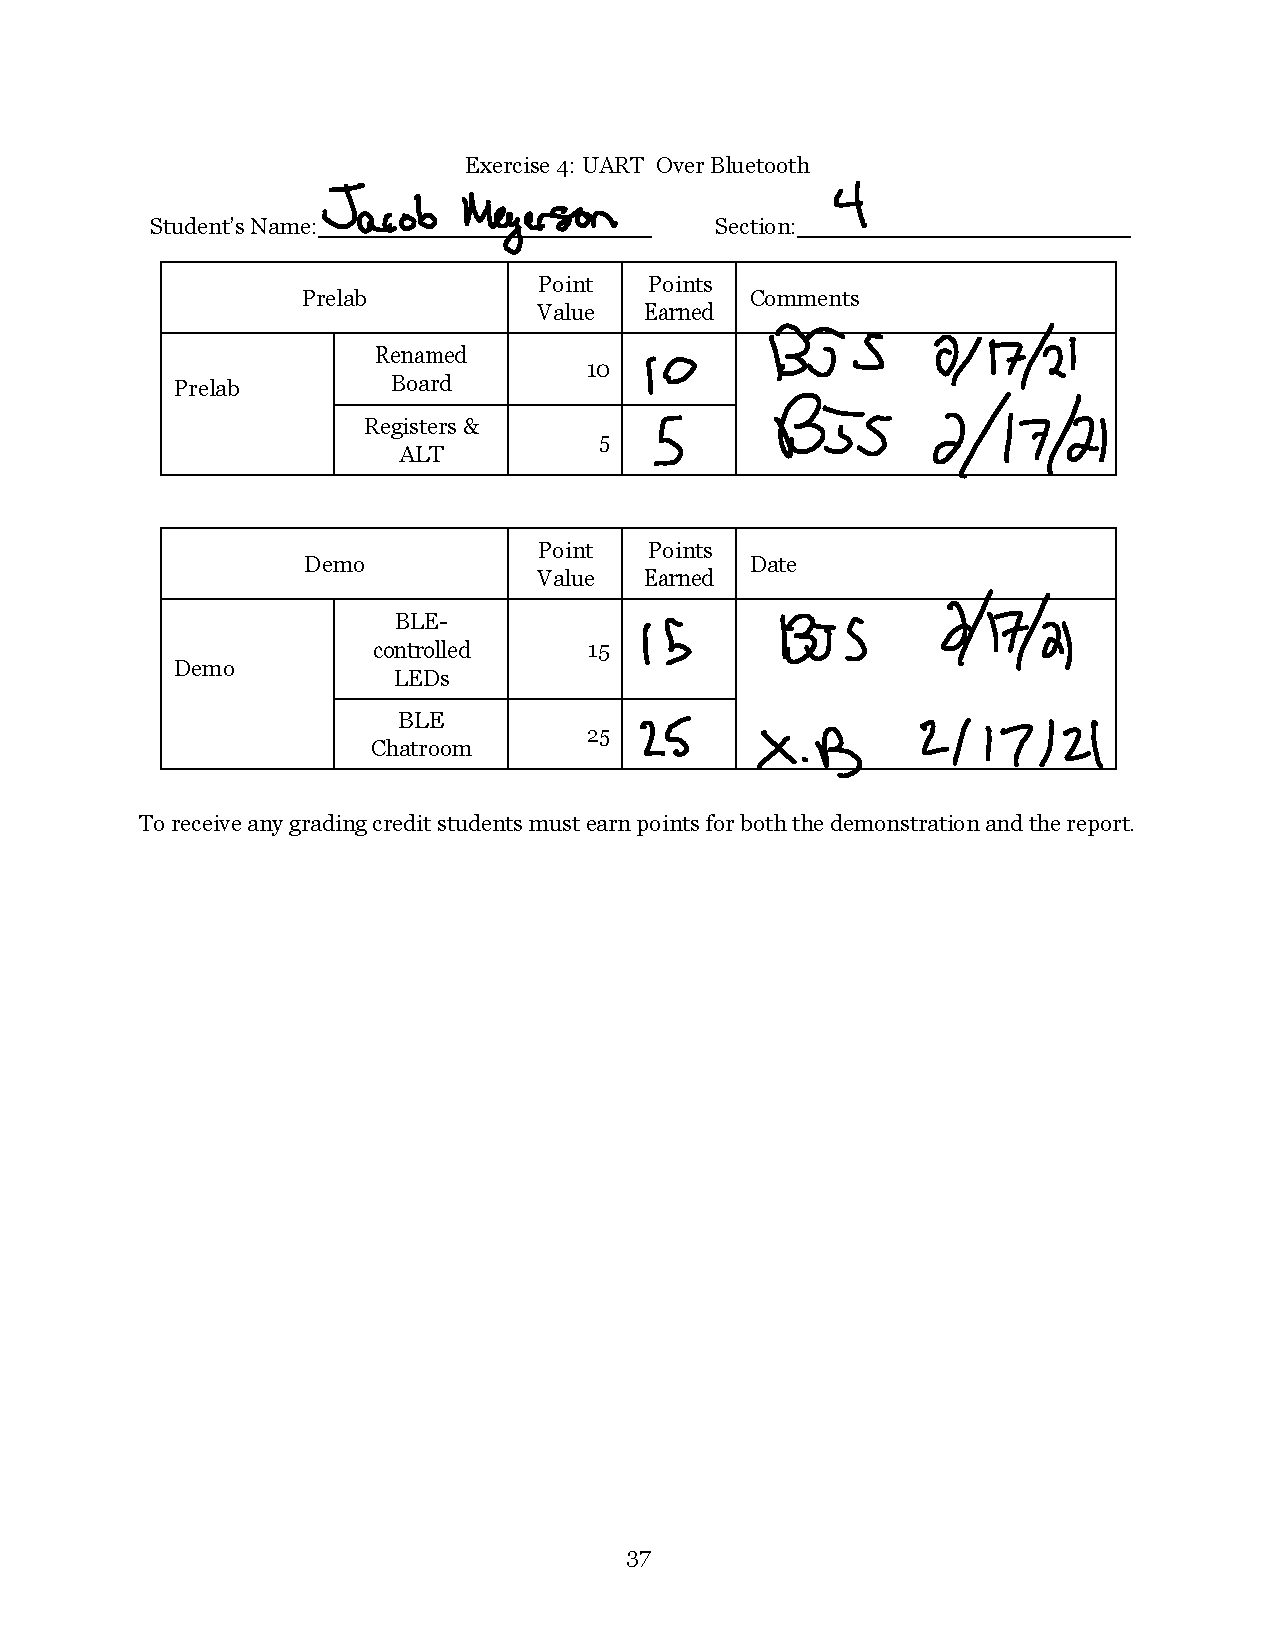
\includepdf[pages=-,pagecommand={},width=\paperwidth]{Screenshots/lab4_signoff.pdf}

\end{document}